% !TEX root = ../../sethomas_thesis_main.tex
\documentclass[border=1mm,
               class=article
               preview]{standalone}
\usepackage{tikz}
% trim={<left> <lower> <right> <upper>}
\begin{document}
\begin{tikzpicture}
    \node[anchor=south west,inner sep=0] (graph) at (0,0) {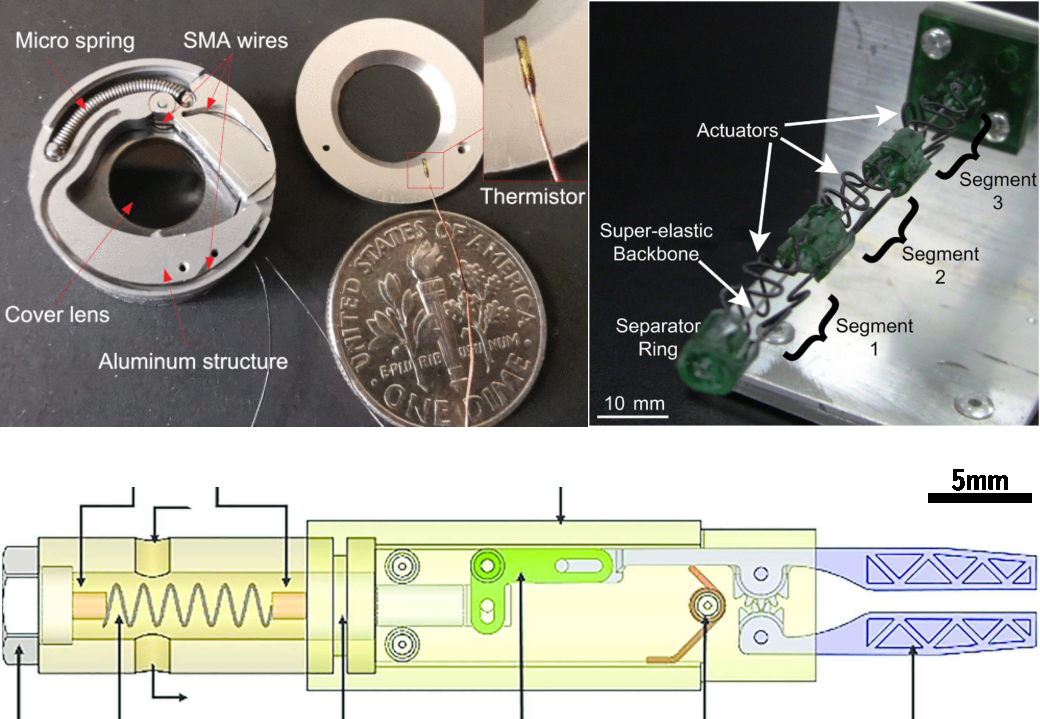
\includegraphics[width=0.7\textwidth]{images/chap1/biomed-examples.pdf}};
    \begin{scope}[x={(graph.south east)},y={(graph.north west)}]
    \node (a) at (0.04,0.46) {\color{white}\textbf{(a)}};
    \node (b) at (0.6,0.95) {\color{white}\textbf{(b)}};
    \node (c) at (0.04,0.37) {\textbf{(c)}};

    \node at (0.02,-0.05) {\footnotesize \makecell[c]{End\\nut}};
    \node at (0.12,-0.05) {\footnotesize \makecell[c]{SMA\\spring}};
    \node at (0.33,-0.02) {\footnotesize Piston};
    \node at (0.5,-0.02) {\footnotesize Link};
    \node at (0.67,-0.05) {\footnotesize \makecell[c]{Steel torsional\\spring}};
    \node at (0.87,-0.05) {\footnotesize \makecell[c]{Gripper\\jaws}};
    \node at (0.17,0.35) {\footnotesize Mount};
    \node at (0.54,0.35) {\footnotesize Base};
    \end{scope}
\end{tikzpicture}
\end{document}
